\documentclass[12pt]{article}

\usepackage{sbc-template}

\usepackage{graphicx,url}
\usepackage{authblk}

\usepackage[utf8]{inputenc}  
% UTF-8 encoding is recommended by ShareLaTex
\sloppy

\title{Team Description Paper of \\
Indian Institute of Technology Kharagpur for IARC}

\author[1]{Somesh Kumar}
\author[2]{Gaurav Gardi}
\author[2]{Manash Pratim Das}
\author[2]{Krishnakant Deshmukh}
\author[2]{Ashwary Anand}
\author[2]{Amit Pathak}

\affil[1]{Professor\\ Depeartment of Mathematics\\Indian Institute of Technology, Kharagpur}

\affil[2]{Students\\ Indian Institute of Technology, Kharagpur}
\renewcommand\Authands{ and }

\begin{document}
\maketitle
\\

\begin{abstract}

\begin{center}\textbf{ABSTRACT}\end{center}
This paper reports the current preparation strategy of Aerial Robotics Kharagpur,
participating in IARC Mission 7 2018. Our main goal includes robust, indoor 
localization in GPS denied environments supported by optical flow sensors. 
Other features like ground i-robots detection and differentiation between the 
target bots and patrol bots is also discussed, followed by a brief description 
of the herding algorithm AI algorithm to be used.
\end{abstract}
\section{INTRODUCTION}
Our research group, Aerial Robotics Kharagpur, started in January 2015 with IARC 
being the prime target. Hence we started on with the problem statement of IARC 
mission 7. Our team was organized into two major domains, which are "controls" 
and "software". Keeping Robot Operating System (ROS) as the base we developed 
our simulation environment in ROS and Gazebo in order to speed up the software 
development and testing while the hardware gets ready. As mission 7 is based 
indoor, hence we made April Tags based indoor true value setup. We have a website[18] 
and a GitHub Organization[19].
\section{SIMULATION}
Gazebo, an open source robotics simulator is used to simulate the robot along with the mathematical, physical and visualization model.It also emulates the environment with the physics and other interactive robots.We have made ROS plugin for the behaviour of i-robots, whereas the quadcopter model,
is made on top of hector\_gazebo, supported by JSBSim, ArduCopter, RotorS,MAVROS,ardupilot\_sitl\_gazebo plugin. For simulations on Pixhawk, we used PX4 SITL after interfacing it with ROS.
\begin{center}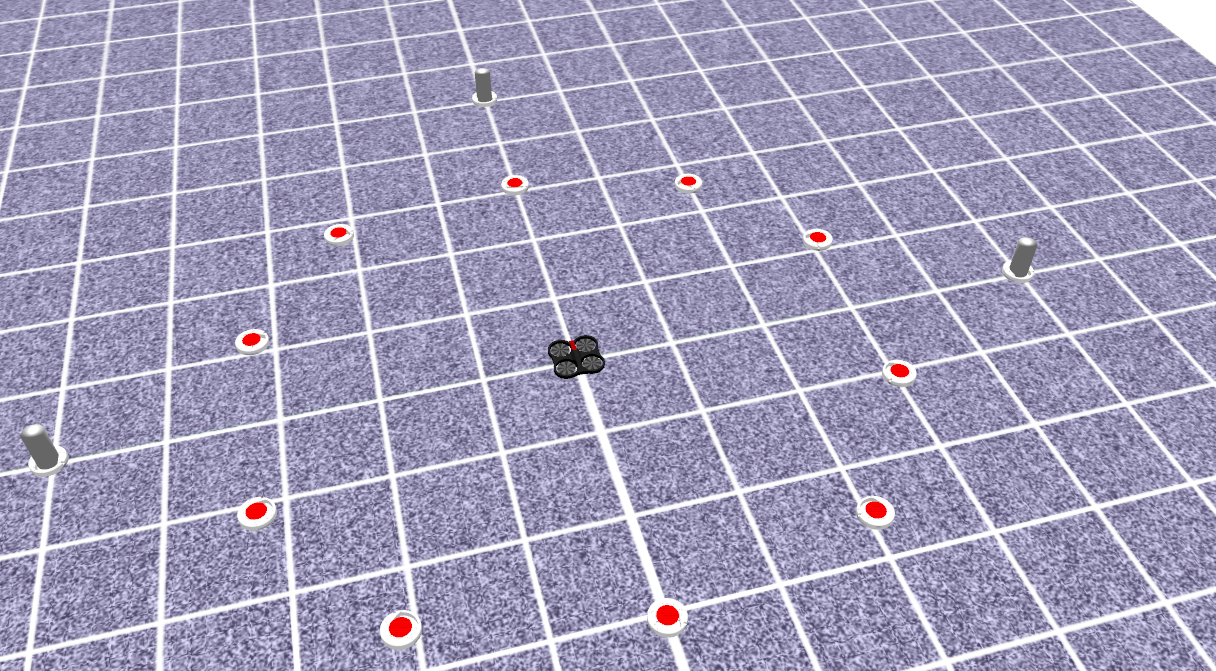
\includegraphics[scale=0.15]{sim} \\
\textbf{Figure 1. Gazebo Simulator.}\end{center}

\section{OVERALL SYSTEM DESIGN}
\begin{center}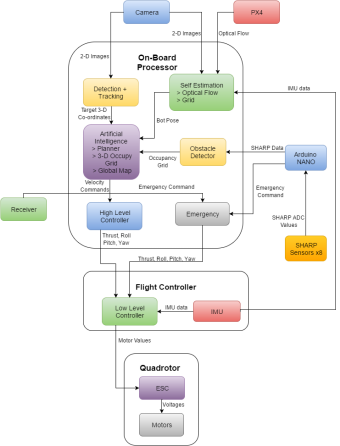
\includegraphics[scale=0.5]{image22} \\
\textbf{Figure 2. System design}\end{center} \\

\section{LOCALIZATION}
We propose a monocular visual localization over grid-lines algorithm for indoor  localization  of  Micro  Aerial Vehicles  (MAVs)  that  is  accurate  and  computationally  fast for  real-time  on-board  processing. Algorithm  explicitly models  the  grid-lines  and  uses  probabilistic  clustering  and labeling  method  to  fit  observed  grid-lines  to  the  model.  A Random sample consensus (RANSAC) method is used to detect outliers and reject the false positive lines before fitting the model.It performs a five degree of freedom (5DoF) localization (position along X, Y, Z axis, roll and pitch) relative to  the  grid-based  floor  in  a  two-step  sequential  process.  The first step involves localizing the MAV within a unit grid cell. Since a grid is a 2D plane of repeating unit cells (rectangles),the  unit  cells  cannot  be  differentiated  from  each  other  when only a partial grid is visible. Hence, the relative positions are integrated using a winner take all (WTA) method in the second stage  to  determine  the  position  estimate  over  the  grid-based floor.

\subsection{Grid Localization}
 In our implementation, we use Hough Transform. Since we can filter out the false positives (outliers), we use Hough Transform  with  threshold  parameters  that  allow  for  more false  positives  than  false  negatives.  Each  line  is  represented by  a  two-element  ordered  set(\rho;\theta).\  $\rho$  is  the  perpendicular distance between the line and the coordinate origin (0;0) (top-left  corner  of  the  image)  in  pixels.  While $\theta$ \  is  the  angle  in radians,  the  normal  to  the  line  makes  with  the X axis  of image.   Let $L_r_a_w$= \{ ($\rho$; $\theta$) \in \  $R^2$ | \rho \geq 0;\ -\pi \ \leq \theta < \ \pi \ \} \   $be the set of all the detected lines.$ 
 \\ 
 $L_r_a_w$ = $L_i_n_l_i_e_r_s$ \bigcup \  $L_o_u_t_l_i_e_r_s$ \ , where $L_i_n_l_i_e_r_i_s$  a  set  of  lines  that  belong  to  grid-lines,  and $L_o_u_t_l_i_e_r$ \ is  the set of lines which are not a part of the grid-lines, as detected from the image. Hence a line is represented by a point in (\rho;\theta) \ space.
\subsubsection{Detecting the Grid}
We  use the  linear  relationship  between $\rho$ and $\theta$ for  a  set  of  parallel  lines,  and  perform  a  Random  Sampling
Consensus  (RANSAC)  with  a  2D  linear  model  on  the  set of  detected  lines $L_r_a_w$ .  RANSAC  is  performed  twice  without replacement  to  get  two  best  fit  inliers  to  the  linear  model , hence  two  best  sets  of  parallel  lines  from $L_r_a_w$ .  Further,  the set  of  parallel  lines  (ordered  set  of ($\rho$ ; $\theta$ )),  with  arithmetic mean  of $\theta$ closer  to 0 is  denoted  as $L_l_o_n_g$ and  that  closer  to $\pi$/2 is denoted as $L_l_a_t$ . Hence, the filtered set of lines $L_f_i_l$ , that contains  only  those  detected  lines  which  belong  to  the  grid-lines (two sets of parallel lines with separation of around $\pi$/2 in  mean $\theta$ )  is  generated  as $L_f_i_l$ = \ $L_l_o_n_g$ \bigcup \ $L_l_a_t$
\\
We use univariate kernel density estimation (KDE)to  estimate  the  probability  density  of $\rho$ in $L_l_a_t$ and $L_l_o_n_g$ individually, as given by \\
\begin{equation*}
\begin{LARGE}
$f_b($\rho$)$ \  = \frac{1}{nb} $\sum\limits_{i=1}^{n}$ K\left(\frac{\rho - \rho_i}{b}\right)
\end{LARGE}
\end{equation*}
\begin{center}
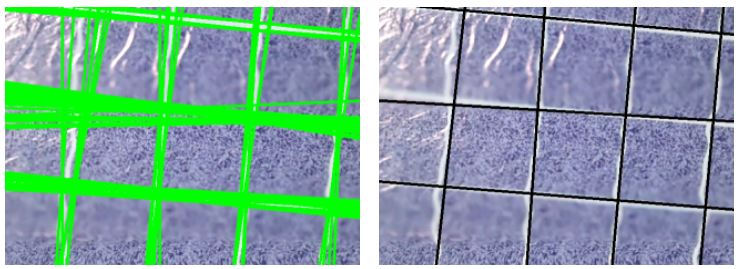
\includegraphics[scale=0.6]{grid2}\\
\textbf{Grid Line Detection}
\end{center}
\subsubsection{Orientation and Cell Localisation}
\begin{itemize}
    \item   In  the $\rho$ ; $\theta$ \ space,  the slopes of the linear curves $m_l_a_t$ and $m_l_o_n_g$ , joining the ordered sets  of  parallel  lines  in $L_l_a_t$ and $L_l_o_n_g$ are  related  to roll ( $\alpha$ ) and pitch ( $\beta$ ) respectively as \\ 
    $\alpha$ = \ $tan^-^1(m_l_a_t)$ \times \  $\epsilon_\alpha$ + $\epsilon_c_\alpha$ \\
    $\beta$ = \ $tan^-^1(m_l_o_n_g)$ \times \  $\epsilon_\beta$ + $\epsilon_c_\beta$ \\ 
    where $\epsilon_\alpha$, $\epsilon_c_\alpha$, $\epsilon_\beta$ and $\epsilon_c_\beta$ are constants obtained from camera calibration.
    \item  We  consider  the  distance  ($s_Y$) between  each  longitudinal line of the grid-based floor and the camera position along $Y_W$ axis.  The  line  to  the  immediate  positive $Y_W$ direction,  with respect to the camera position is indexed as i = 0.
    \item The projection of any line of magnitude c in $Y_W$ axis with camera position as the origin is given by g(c) \\ 

    $\textit{g(c)} = \left(\frac{{c \times cos(\phi_Y) \times f}}{cos(\delta)\times h}\right) $
    \item Squared L2 error cost function is used to estimate sub cell position and height based on observed \rho .
\end{itemize}
\begin{center}
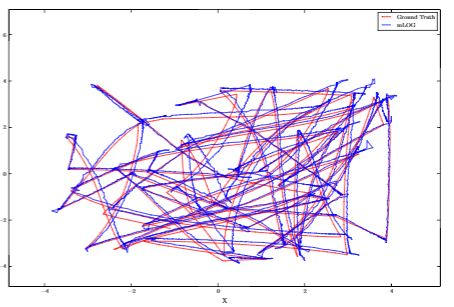
\includegraphics[scale=0.6]{grid}\\
\textbf{Localization and True Value}
\end{center}}
\subsubsection{Grids Localization}
Let $\sigma_k^Y$ be  the  position  within $u_k$ unit  cell  and $p^k_Y$ be  the position  of  the  MAV  with  respect  to  an  initial  position  over the grid-based floor at $k^t^h$ frame. Hence we have \\
$u_k$ = $\left(\frac{p^k_Y}{m_Y}\right)$ \\
At $(k + 1)^t^h$ frame, the new sub-cell position $\sigma^k^+^1_Y$ , might be from $u_k_-_1$ ,$u_k$ or $u_k_+_1$ unit cell, considering the maximum MAV speed is limited. Hence three possible position of the MAV at $(k + 1)^t^h$ frame are $P_Y$ = $\{(p_Y_- 1);(p_Y);(p_Y + 1)$ \\
where $p_Y$ = $p^k_Y$ + $\sigma^k^+^1_Y$ - $\sigma^k_Y$. The MAV’s new position $(p^k^+^1_Y)$ is given by a winner take all (WTA) scheme, decided by $p^k^+^1_Y$ = $argmin(p^k_Y - p^'$$_Y )^2$
\section{GROUND ROBOT DETECTION AND TRACKING}
    \subsection{Detection}
        \subsubsection{Ellipse Detection}
            \begin{itemize}
                \item The detection of each Ground bot will be done with a modified form of Randomized Hough Transform(RHT), fully described in reference, to detect ellipses that correspond to the edges of the bots. 
                \item Two points are selected as the ends of a major axis, and a third point on the assumed ellipse is selected randomly and the vote of the accumulator is done on the length of the minor axis.          
            \end{itemize}
    \begin{center}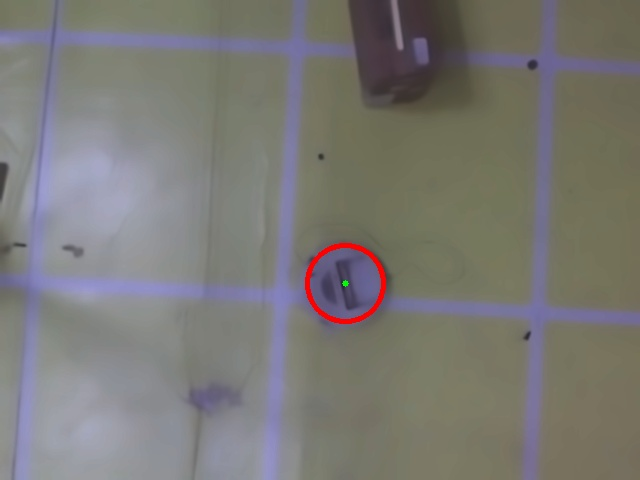
\includegraphics[scale=0.2]{Pic2} \\
    \textbf{Bot Detection using Ellipse Detection for downward facing camera}\end{center}
        \subsubsection{YOLO Based Object Detection}
            \begin{itemize}
                \item Modified R-CNN as described in YOLO is trained on 40,000 images of the iRobot taken from different angles and height to detect the ground bot at steep angles where the ellipse method fails to detect the ground bots because of very high eccentricity of the viewed bots.
            \end{itemize}
    \begin{center}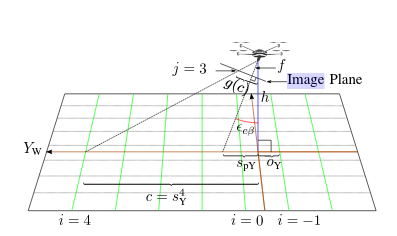
\includegraphics[scale=0.44]{trig} \\
    \textbf{Trignometric pose estimation from front camera}\end{center}   
    \subsection{Position Estimation}
        Once the bots are detected, the noise associated with the dynamic observables of the moving bot will be filtered out using a Kalman filter to enable tracking of the bot.  This is achieved by the following steps:
        \begin{itemize}
            \item The Kalman Filter takes in the measured position of the bot(which in this case is the centre of the ellipse detected by the RHT) as well as its velocity from the video feed.
            \item The position can also be estimated by mapping the image to real frame using simple pin hole camera model and trigonometry. Position of the ground bots are measured with respect to the current position of the quad for known camera configurations.
            \item Downward facing camera runs the ellipse detection code only as it will remain perpendicular to the ground thus the pitch will be negligible.
            \item Front facing camera runs YOLO object detection to detect ground bots for steeper angles.
            
            \item The error associated with each of these quantities is also found by calculating the expected noise in the readings. The error is estimated as a Gaussian function. 
            \item These two quantities (measured and predicted positions) are compared and the best guess of the bot’s position is made by considering it to be the configuration for which both estimates are most likely after incorporating the associated errors.
        \end{itemize}
    
    \subsection{Tracking of Multiple Robots}
        \begin{itemize}
            \item Having found the most probable position of each bot using the Kalman filter, the next step is to track multiple bots.
            \item A cost matrix is created which incorporates the direction in which the bots had been moving, the distance of the updated estimates of positions from the previous estimates, the expected collisions as well as the expected turns.
            \item The cost matrix is run through the Hungarian algorithm to associate the updated positions with the previous positions, thus giving an identity to each bot, and enabling multiple bot tracking.
        \end{itemize}

\section{OBSTACLE AVOIDANCE}
    IARC consists of moving obstacle robots which need to be avoided when they are on the way of the desired trajectory and path.
    \\ \\
    Obstacles Description: 4 Ground Robots with cylinders attached on top of them to form vertical moving obstacles.
    \\ \\ 
    \textbf{Avoidance Algorithm Overview:} \\
    The Obstacle Avoidance in IARC does not need to be global as the number of obstacles are less in number. So, we use 1-dimensional Lidar attached to a stepper motor to cover 360 degree obstacle detection. If the obstacle is closer than a threshold then multiple kinds of action can be taken:
    \begin{itemize}
        \item Wait for Obstacle to Move out of Path
        \item Avoid Obstacle by Creating a New Trajectory around the obstacle and come back to desired trajectory.
    \end{itemize}
        \subsubsection*{Procedure I:}
            \begin{itemize}
                \item Interrupt Control is triggered as soon as an obstacle comes closer than 40cm from the Lidar.
                \item Depending on orientation of the obstacle with respect to Lidar and comparing with velocity direction of robot, the robot is halted at the same position or commanded to follow line in reverse till last node is found.
            \end{itemize}}
        \subsubsection*{Procedure II:}
            \begin{itemize}
                \item Trajectory Generation Module is used to generate trajectories from node to node via the lines or directly.
                \item This trajectory generation is recalculated on obstacle trigger and a visible graph is created around the obstacle and followed till next grid node.
            \end{itemize}

\section{SYSTEM CONTROL}
\subsection{Pixhawk}
    We have used Pixhawk 2.0 which runs the PX4 v1.6.0 firmware. PX4 is a nearly feature-complete open source UAV firmware. Thus our high level control is utilizes the features of PX4 to its fullest. Since, most of PX4’s autonomous features uses GPS, we used motion capture system to get position data from other sources like vision. Position estimates were sent from an onboard computer. This data was used to update its local position estimate relative to the local origin.  
\subsection{MAVROS}
    Since Pixhwak communicates in Micro Air Vehicle Link(MAVLink) protocol and both our ground station and onboard computer uses Robot Operating System(ROS), we used MAVROS for communication between onboard computer and Pixhawk. MAVROS is a MAVLink extendable communication node for ROS.
\subsection{Ground Robot Tapping}
    We use a vertical descent strategy, making our MAV go to a desired location ahead of the ground bot ,at a certain default height and then make it descend such that the descent takes the same amount of time as the ground bot to reach these desired coordinates on the ground. \\
\\ Assuming a right handed Cartesian coordinate system \\
\begin{center}
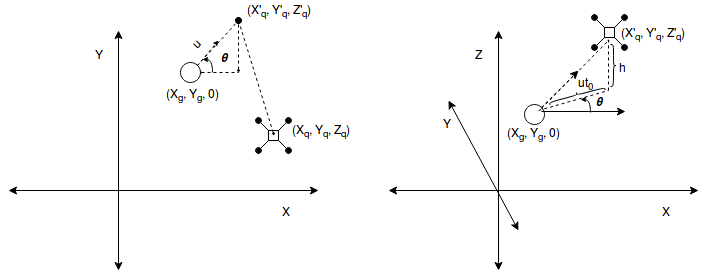
\includegraphics[scale=0.3]{tap}\\
\textbf{Tapping Mechanism}
\end{center}
Let,
    
u = velocity of the ground bot in the direction of its motion 

$\theta$ = orientation of the ground bot with respect to x axis 

$(X_g, Y_g, 0)$ = coordinates of the ground bot 

$(X_q, Y_q, Z_q)$ = Coordinates of the MAV 

($X_q^’$, $Y_q^’$, $Z_q$) = Desired Coordinates of the MAV before it starts to descend 

Where $Z_q$ = $h$ = Default height we want for the MAV in order to avoid obstacles 
        
$t_0$ = time required by MAV to descend from the default height 
 
Calculating the desired coordinates for the MAV, 
 
$X_q^’$ = $X_g + ut_0cos(\theta)$

$Y_q^’$  = $Y_g + ut_0sin(\theta)$ \\
    As soon as the MAV reaches these desired coordinates, it starts descending, vertically. In the same time the ground bot reaches these desired coordinates, making the tap successful. 
    Our only assumption in the method is that the velocity of MAV is greater than the velocity of ground bot. It is ensured by the low level controller that this condition is always satisfied.
\section{IARC ROBOT DESCRIPTION}
\begin{center}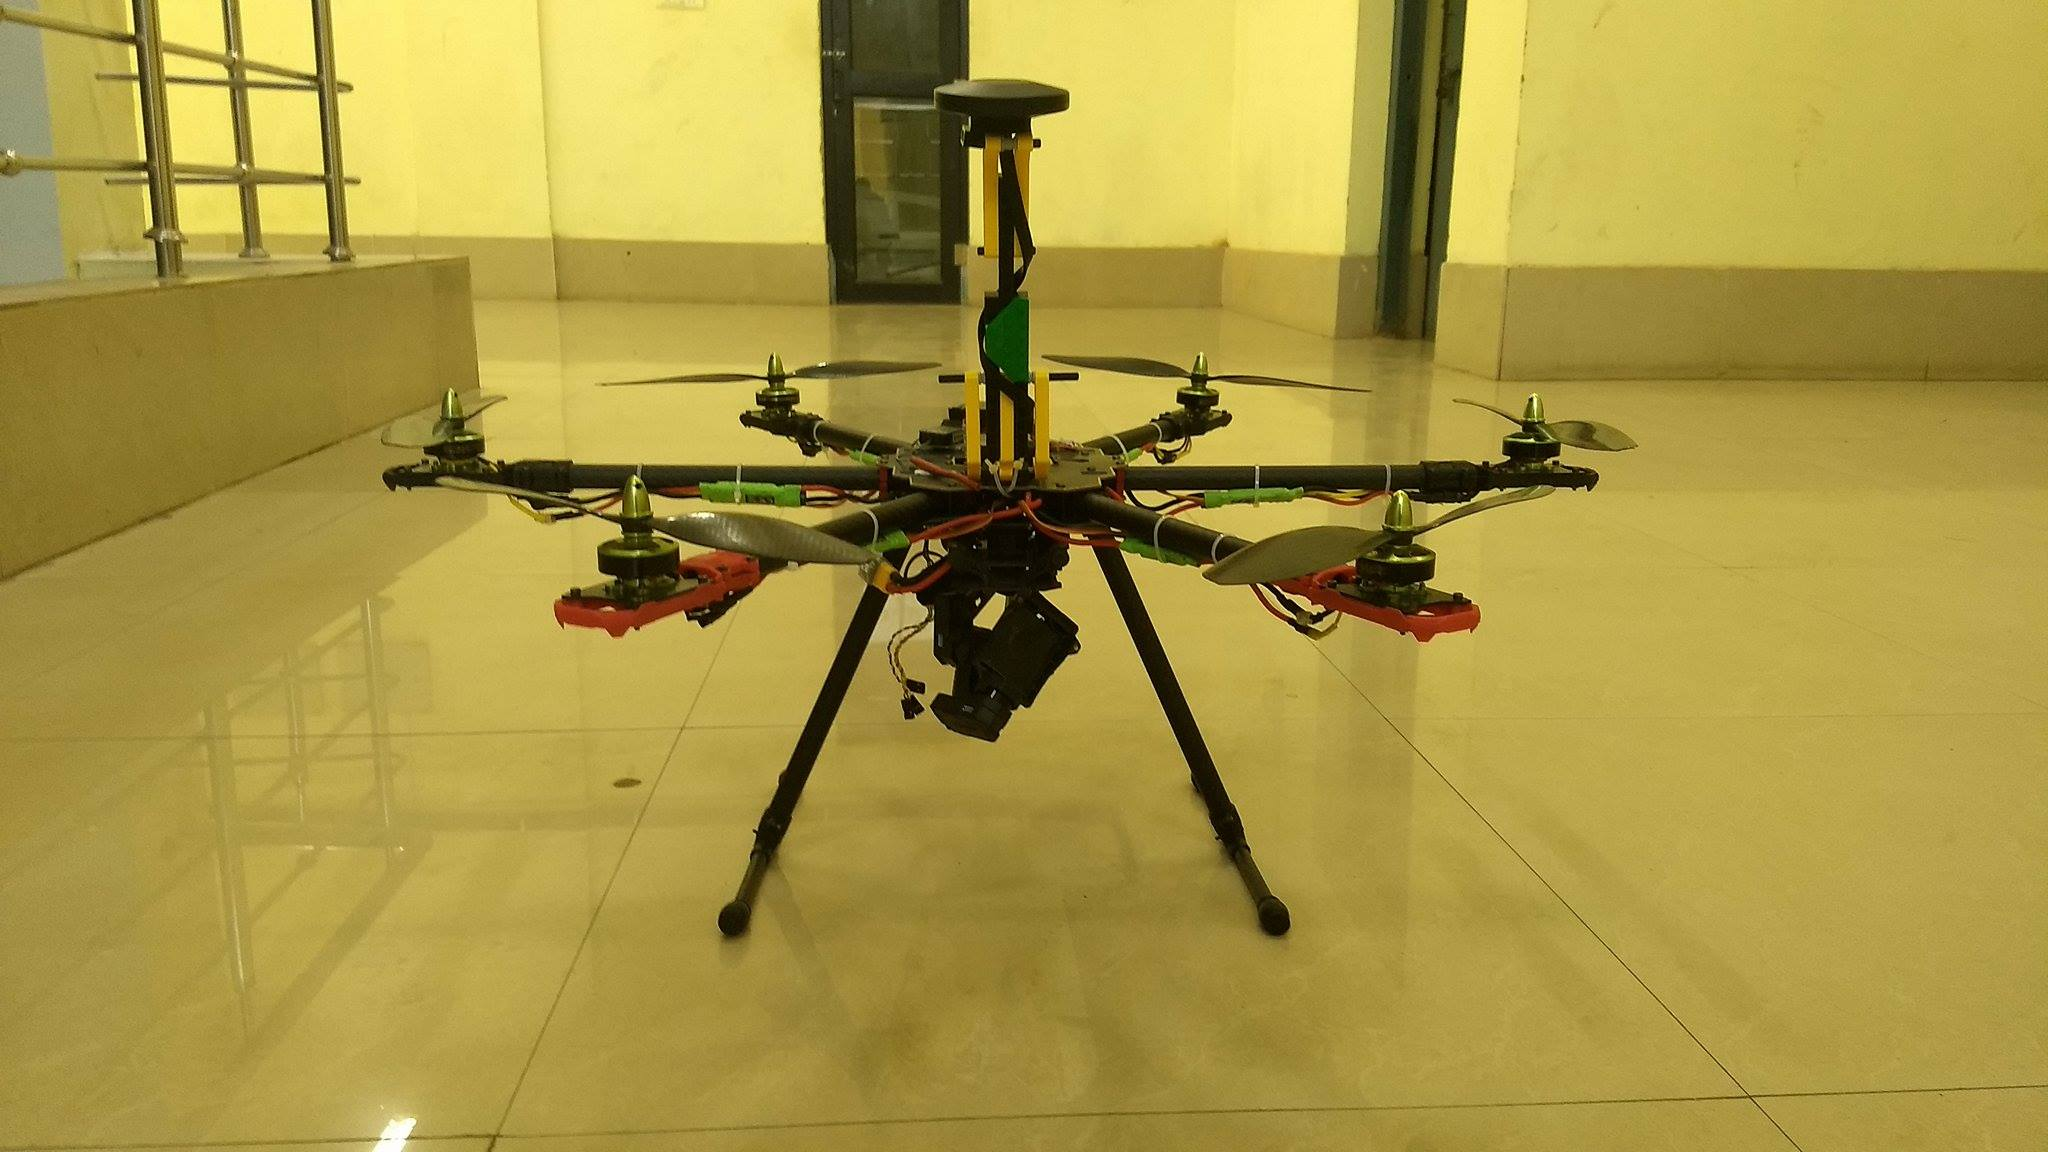
\includegraphics[scale=0.15]{hex} \\
\textbf{Figure 8. Hexcopter}\end{center}\\
\subsection{Configuration}
\begin{itemize}
    \item Odroid XU4 : High Level Controller
    \item Pixhawk 2.0 : Low Level Controller
    \item ESC     : Electronic Speed Controller, 45A OPTO
    \item LiPo     : 11.1V, 3s, 6000mAh, 35C
    \item Motors: 850kv BLDC
    \item Propellers : 11” x 4.7”
    \item Camera Front: 30fps, Field of View - 78 degrees, Aspect Ratio - 16:9
    \item Camera Downward: 30 fps, Field of View - 170 degrees, Aspect Ratio - 16:9
    \item Receiver : 6 channel PPM, PPM Encoder
    \item Frame : HMF S680 Hexacopter
\end{itemize}

\section{HERDING ALGORITHM AI}
\subsection{Greedy Method}
\begin{itemize}
    \item The motif of this algorithm is to make as many bots cross the green line as possible with a fixed radius around the ground bot in which all the other bots will be herd with the centre bot towards the green line.
    \item Before takeoff, the hexacopter will be fed with the direction information about the green and red lines. The direction information will tell where is the red line (east/west/north/south).
    \item Once the hexacopter takes off, it will hold altitude at 1.5m (from ground) and hold position on the nearest node while holding its yaw.
    \item It then follows the grid to:
        \begin{itemize}
            \item Detect the position of lines.
            \item Follows the grids to scan for the ground bots.
            \item Scan for the bots such that to reduce their variance below certain limit.
        \end{itemize}
    \item The hexacopter will now start to locate the closest bot to the green line.
        \begin{itemize}
        \item If ground bots are found in the herding radius of the centre bot, then it will herded with the centre bot towards the green line keeping them inside the circle of specified size. 
        \item Once the centre bot crosses the green line, new centre bot among the herd is chosen and the loop is repeated.
        \end{itemize}
\end{itemize}

\section{EMERGENCY KILL SWITCH}
\begin{itemize}
\item One Dual-D flip flop CD4013B, 5 IRF540N MOSFETs, capacitors and resistors are used. We used the receiver’s signal as source to the circuit which is equivalent to the Pulse generator with variable duty cycle shown in the circuit. The leftmost MOSFET is a controller and the rest 4  mosfets  are connected in series with the negative terminal of LIPO(power source). 4 MOSFET in parallel to each other are used  keeping in mind that each can take a max of around 33 Amps and combined will allow max of around 132 Amps for a quadrotor. For Hexacopter 7 MOSFETs should be used, one as a controller MOSFET and the rest 6(parallel to each other) in series with negative terminal of the power source/LIPO. 6 MOSFETs ensure that max current allowed for the bot is raised to around 190 Amps.  
\item Below a particular duty cycle(T) the controller MOSFET has $V_g_s$<$V_t_h$ and will go in cutoff region as shown below leading zero drain current in it and potential drop across its drain resistor as a result rest MOSFETs will have Vgs=5V due to which they go in saturation region and with very low Vds and in this mode the bot is supplied with power source.\\
\begin{center}
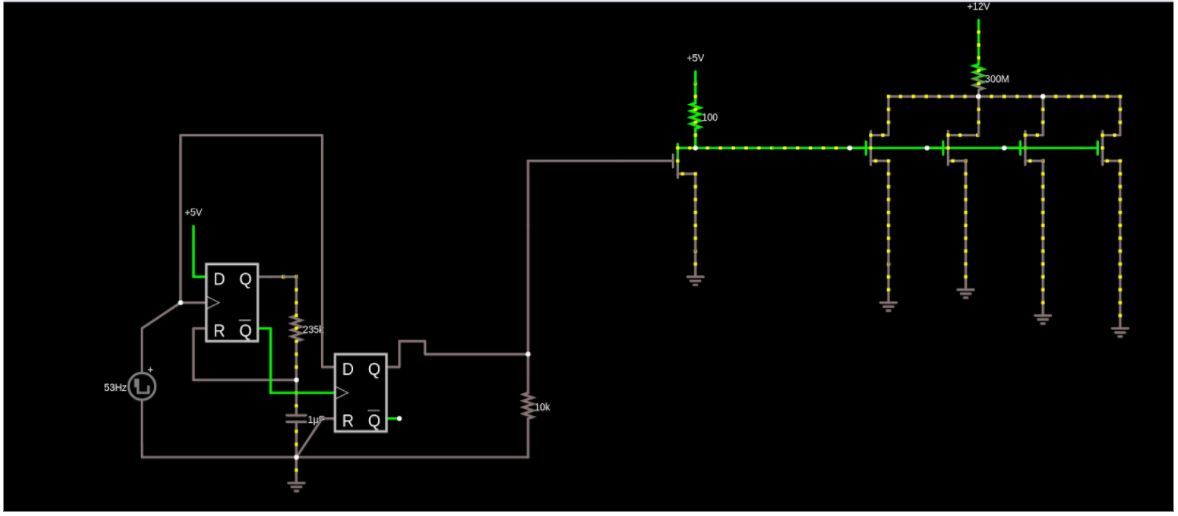
\includegraphics[scale = 0.4]{kill} \\
\textbf{Kill Switch Circuit}\\ \\
\end{center}
\\
\item Above a particular duty cycle(T) the controller MOSFET has $V_g_s$>$V_t_h$ and will go in saturation region and as a result rest MOSFETs will have $V_g_s$ = 0V due to potential drop across drain resistor of controller MOSFET and this will make the rest MOSFETs go in cutoff region as a result cutting of the negative terminal from battery and hence no power supply to the bot. The whole system shuts down instantly.
\item Duty cycle(T) or as in our case PWM of signal  sent through the transmitter at which the bot is killed can be varied by varying the capacitor’s value.The bot is represented here as the 300 milliohms resistor as there was no way to symbolize the actual bot.
\end{itemize}

\section{TESTING}
\begin{center}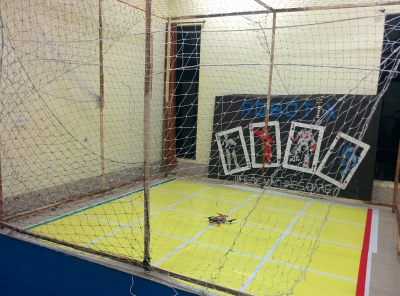
\includegraphics[scale=0.7]{ARK-lab-kgp1} \\
\textbf{Figure 11. Sample testing arena}\end{center}\\
We have an indoor testing arena with sample grid floor as in IARC arena and two iRobots. We have safety harness to 
tie up the quadcopter while testing various controls and PID tuning. \\
We tested the AI (Herding) algorithms on the simulator. We tied the quadcopter with various allowed degree of 
freedom to test altitude hold, yaw hold, node hold and grid following algorithms on the real quadcopter and hexacopter in our arena.
\section{State Machine}
\subsection{States}
\begin{itemize}
\item {Find/ Scan : Quad roams in the arena searching for bots and saving their location.}
\item{Bot Prediction : Predicts the best bot to attack and return its position}
\item{Obstacle Avoidance : Avoids the obstacle}
\item{Strategy : Plans the path and way the bot must be attacked.}
\end{itemize}
\subsection{Working}
\begin{itemize}
\item{Once the take off is successful the control is passed to the FSM. Entry point in the FSM is the Find / Scan state. In find state quad tries to localize itself as well as search for the bot. Detection and localisation is based on probabilistic models including gaussian errors.
}
\item{Quad stays in find state until the probability of bot(s) doesn't increase a certain threshold , let's say K%.
}
\item{Once quad is certain about the position of bot(s) with probability greater than K , control is passed to Bot Prediction state which predicts the bot which should be attacked among the bots with certainty higher than K% and sends the location of the bot to Strategy state.
}
\begin{center}
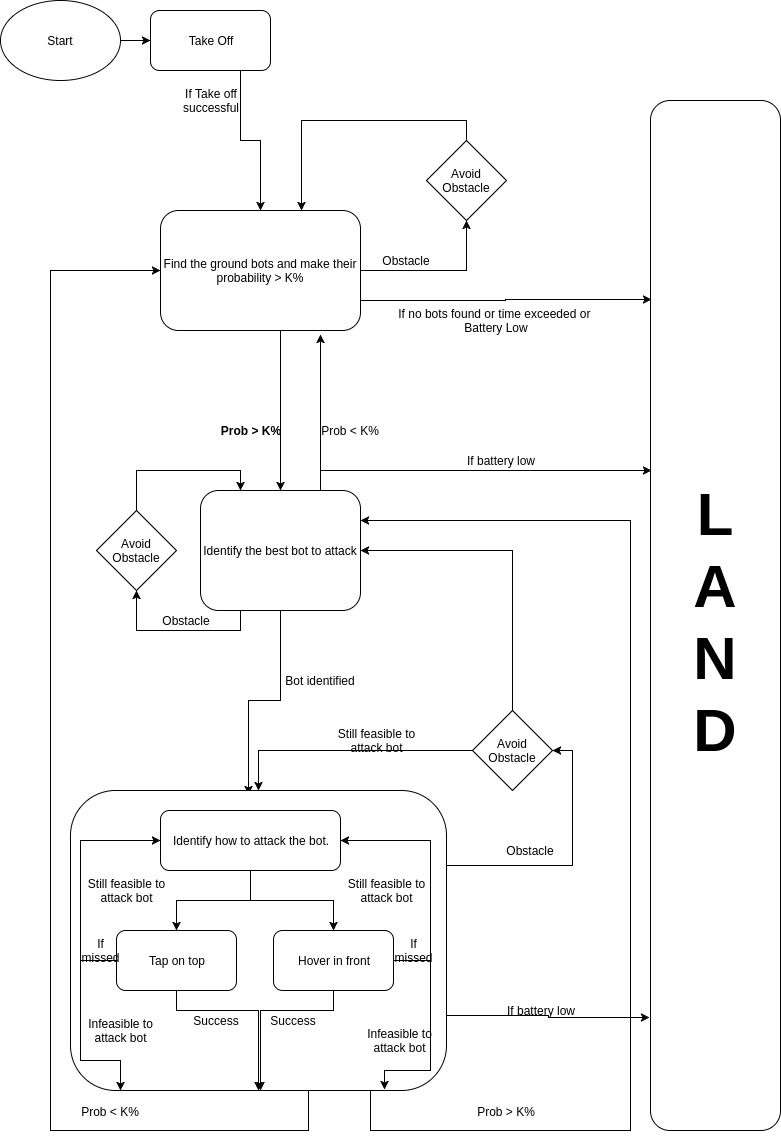
\includegraphics[scale=0.4]{st_mcn} \\
\textbf{State Machine Diagram}\end{center}\\
\item{Strategy state tries to analyze the different states of the bot like position, velocity and direction and accordingly decides how the particular bot should be attacked.
}\\
If any of the two method fails to execute properly and the probability of the current bot is still high and feasible to attack the state is looped to re-determine the best way among two to again attack the bot, else control simply shifts to bot prediction mode to identify the next best bot to attack.
\end{itemize}
\subsection{Rules}
\begin{itemize}
\item{State interrupted is re-run after obstacle is avoided excluding the Strategy state where a check redirects it to Strategy or Bot detection state according to the feasibility of attacking the same bot again.
}
\item{Anytime the probability of bot(s) go below the K, state will shift to Find / Scan to increase the certainty of the bot(s). Exceptions :
}
\begin{itemize}
\item{Quad is attacking one bot with high certainty : A threshold delta must be considered in such conditions when the probability of other bots is allowed to fall as low as K-delta % as attacking the bot may increase our points.
}
\end{itemize}
\item{Battery is given the highest priority of all. If the battery is low , state machine will be terminated and the quad will land.
}
\end{itemize}
\section{References}
\begin{enumerate}
        \item \href{https://books.google.co.in/books?id=4YCThwzeTBQC&redir_esc=y}{\textit{E. L. Houghton, P.W.Carpenter} Aerodynamics for Engineering Students. 
    \item \href{https://books.google.co.in/books/about/Fundamentals_of_Aerodynamics.html?id=CaBTAAAAMAAJ}{$\textit{John David Anderson}$ Fundamentals of Aerodynamics. }}
    \item \href{https://books.google.co.in/books/about/Fundamentals_of_Compressible_Flow.html?id=_NCz9iZIugYC}{\textit{S. M. Yahya } Engineer's Aerodynamics. }
    \item \href{http://eprints.qut.edu.au/33732/1/cep2009_modelling_and_control_paper_sub_final.pdf}{\textit{P. Pounds, R. Mahony, and P. Corke} Modelling and Control of a Large Quadrotor Robot. }
    \item \href{http://ieeexplore.ieee.org/iel5/5076472/5152175/05152390.pdf?arnumber=5152390}{\textit{P. Pounds and R. Mahony} Design principles of large quadrotors for practical applications. }
    \item \href{https://www.researchgate.net/publication/220474158_Towards_autonomous_indoor_micro_VTOL}{\textit{Samir Bouabdallah, Samir Bouabdallah and Roland Siegwart} Towards autonomous indoor micro VTOL. }
    \item \href{http://www.itcon.org/cgi-bin/works/Show?2012_12}{ \textit{Javier Irizarry, Masoud Gheisari and Bruce N. Walker, Associate} Usability assessment of drone technology as safety inspection tools.}
    \item \href{http://www.engadget.com/2011/04/21/t-hawk-uav-enters-fukushima-danger-zone-returns-with-video/}{ T-Hawk UAV enters Fukushima danger zone, returns with video. 6:48PM April 21, 2011, retrieved on April 22, 2011.}
    \item \href{http://9to5mac.com/2011/06/15/awesome-use-of-an-ipad-and-the-parrot-ar-drone/}{\textit{Zibreg. C. (2011)} Awesome use of an iPad and the Parrot AR Drone. }
    \item \href{http://robotics.felk.cvut.cz/faiglj/thesis/papers/icr10.pdf}{\textit{Jan Faigl,  T Krajnık,  V Vonásek,  L Preucil} Surveillance Planning with Localization Uncertainty for UAVs. }
    \item \href{http://ieeexplore.ieee.org/xpl/articleDetails.jsp?reload=true&arnumber=6005280}{ \textit{Wai Shan Ng and Ehud Sharlin} Collocated interaction with flying robots.} 
    \item \href{https://www.researchgate.net/publication/220947254_Flying_sports_assistant_External_visual_imagery_representation_for_sports_training}{\textit{Higuchi, K., Shimada, T., and Rekimoto, J.} Flying sports assistant: external visual imagery representation for sports training.}
    \item \href{http://www.aviationsystemsdivision.arc.nasa.gov/publications/hitl/rtsim/Toms.pdf}{\textit{T. S. Alderete, NASA Ames Research Center, Moffett Field, California.} Simulator aero model implementation.}
    \item \href{https://www.researchgate.net/publication/228962656_Nonlinear_observer_design_and_sliding_mode_control_of_four_rotor_helicopter}{ \textit{ H. Bouadi and M. Tadjine} Nonlinear observer design and sliding mode control of four rotors helicopter.}
    \item \href{https://april.eecs.umich.edu/papers/details.php?name=olson2010tags}{\textit{Edwin Olson} AprilTag: A robust and flexible multi-purpose fiducial system.}
    \item \href{https://pjreddie.com/darknet/yolo/}{\textit{Redmon, Joseph and Farhadi, Ali (2016)} YOLO9000: Better, Faster, Stronger \textit{arXiv preprint arXiv:1612.08242}}
    \item \href{http://wiki.ros.org/px4flow_node}{px4flow\_node}
    \item \href{http://quadrotor-iitkgp.github.io/}{Aerial Robotics Kharagpur: Website}
    \item \href{https://github.com/quadrotor-IITKgp}{ Aerial Robotics Kharagpur: GitHub organization}

\end{enumerate}
\end{document}
